%!TEX root = report.tex

\section{Introduction}
%sentiment analysis
Sentiment analysis is one of the important task in natural language processing community[8] which help people navigate the huge amount of user-generated content available online. Machine learning systems that make decision on the attitude of viewpoints to be positive, neutral or negative that enable people to understand the enormous body of opinions on the Internet, ranging from product reviews to political positions. 

%social network
Interestingly, most of the viewpoints nowadays can be obtained from online website that actually has a social network behind it, since user-generated content often appears in the context of social media. Therefore nowadays user-relationship information is now more easily obtainable. For example, huge amount of tweets from Twitter express people's opinions on different subjects. Each tweet is associated with a user and users formed social network structure through the mechanisms of ``follower''. When a user forms a link in the network such as Twitter, they tend to have a personal relationship then the principle in language called ``homophily'' suggests that users who are connected via some social relationship may also share similar opinions or linguistic variation(each community may have their own ``jargon'' in expressing ideas and sentiments. ). Figure 1 from [1] gives an example of how users from different communities may understand the word ``sick'' differently.

\begin{figure}[h]
\centering
\begin{minipage}{.5\textwidth}
  \centering
  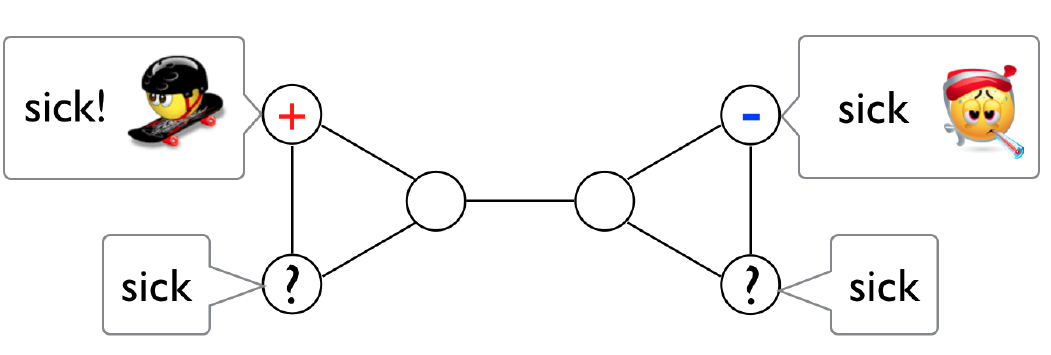
\includegraphics[width=1\linewidth]{sick}
    \label{fig:test1}
\end{minipage}%
\begin{minipage}{.5\textwidth}
  \centering
  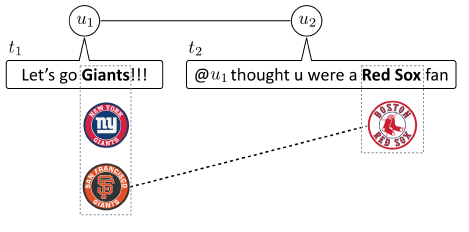
\includegraphics[width=1\linewidth]{Giant}
  
  \label{fig:test2}
\end{minipage}
\caption{Words such as ‘sick’ can express opposite sentiment
polarities depending on the author; Leveraging social relations for entity
disambiguation.}
\end{figure}

\begin{figure}[h]
\centering
\begin{minipage}{.5\textwidth}
  \centering
  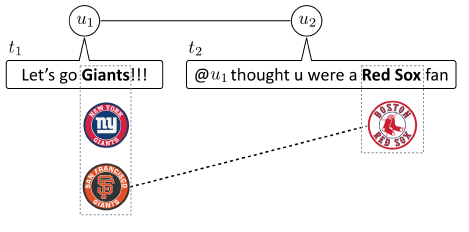
\includegraphics[width=1\linewidth]{Giant}
  \caption{Illustration on leveraging social relations for entity
disambiguation. Socially connected users u1 and u2 tend to
talk about similar entities (baseball in the example).}
  \label{fig:test2}
\end{minipage}
\end{figure}


Nowadays, models that combine social network information with machine learning classification task are proposed in many literature. However, these models rarely utilize the state-of-art deep learning methods like convolutional neural network or network node embeddings which are common in social network and NLP communities. Previous research either use traditional machine learning methods to incorporate social network structure information as in [7] or they separate the textual and user information to build seperate deep learning model as in [8]. In this paper, we are going to explore different methods that utilize jointly social network information and textual information in sentiment analysis with one joint deep learning model that takes both social network information and textual information as input to classify the sentiment of sentences.

Our paper is structure as follows: section 2 will introduce related work to our task and how we relate them; section 3 will define the problem formally and introduce our dataset; section 4 will introduce our model and intuition; section 5 will demonstrate our numerical result; section 6 will discuss our result and draw our conclusion.
